\section{Current view of future detectors}

The individual components of the budget of the total noise of the detectors indicate in which direction research and development of the detector subsystems have to move.

\begin{figure}[h]
%\centering
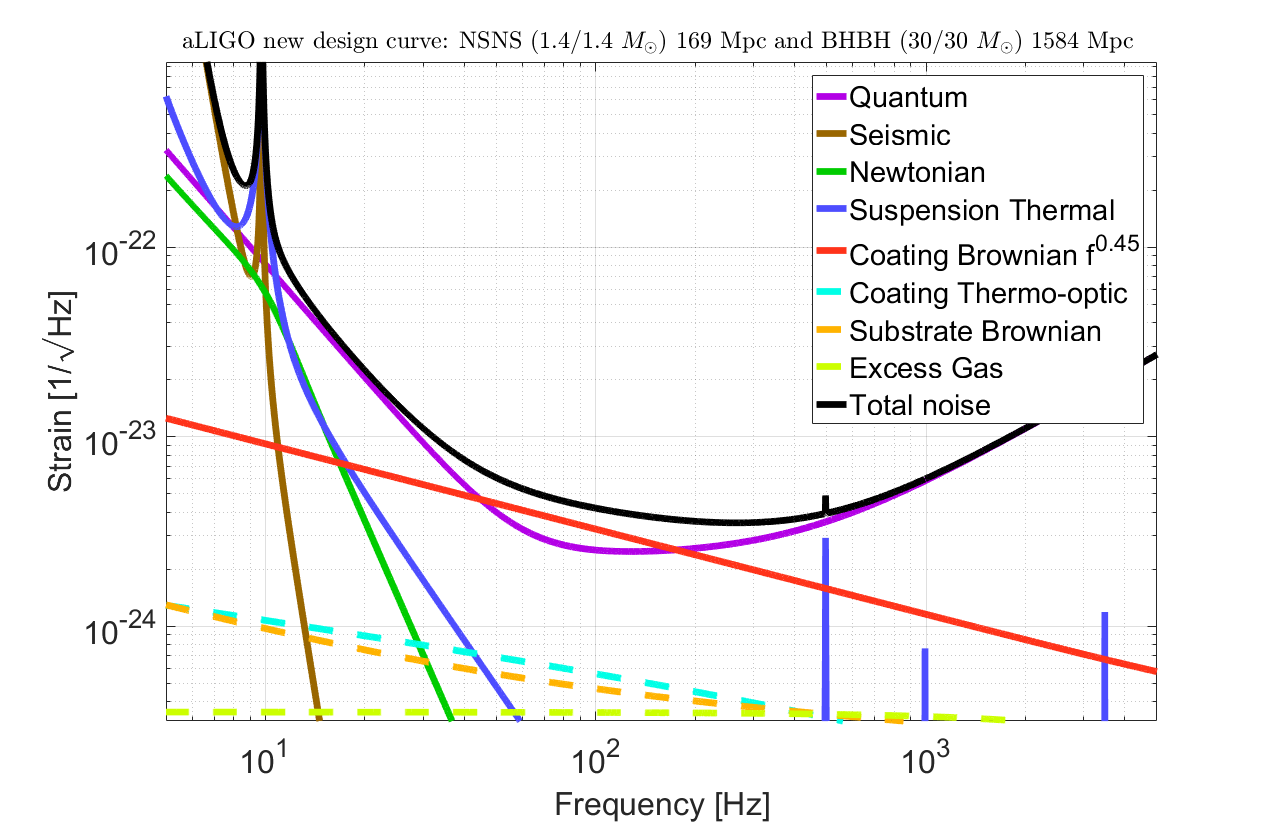
\includegraphics[width=\textwidth]{Figures/aLIGO_newDesign.png}
\label{fig:ALIGOSensitivity}
\caption{Advanced LIGO Noise budget from LIGO DCC T1800044-v4}
\end{figure}



At low frequencies, the sensitivity of current detectors is limited by a variety of noise sources. The ground seismic couples to the mirrors through the seismic isolation platforms and the suspensions.The seismic isolation concepts currently used are expandable and then sufficient for the next generation of detectors. Gravity gradient noise already plays a limiting role in today's detectors at times with increased seismic. Since there are no concepts to prevent or reduce the Newtonian coupling of seismic ground motion to the mirrors, the solution can only lie in a reduction of the ground motion itself or in a measurement and subsequent subtraction of the contributions. Suspension thermal noise, quantum radiation pressure noise, scattered light noise, alignment noise, and a variety of other not yet determined noise sources contribute to the total noise budget in the low-frequency range.
In the high frequency range the sensitivity can be improved by increasing the circulating light power in the interferometer arms and by using squeezed light with a high squeezing level. Both approaches put extreme demands on the optics. Increasing the laser power in the interferometer arms requires extremely low absorption, as due to local absorption of laser light and heating of the optics thermal effects could otherwise negatively affect the performance. Thermal compensation systems will have to be improved to reach the goals of future detectors. Increased light power also increases quantum radiation pressure noise. Due to the higher susceptibility of the mirrors to forces at low frequencies, radiation pressure noise is particularly effective in the low-frequency range. This can be counteracted on the one hand by increased mirror masses, and by frequency-dependent squeezing on the other. Increasing the squeezing level requires extremely low-loss optics, both in the interferometer arms and at the detection port, i.e. between the squeezed-light source, the interferometer, and the photodetector. The optical methods necessary for the rotation of the squeezing ellipse are not yet mature, both with regard to the technical implementation and control methods to be used. High light power in the interferometer arms can lead to parametric instabilities. These will already play an important role in the final stage of the current advanced detectors. The suppression mechanisms, e.g. with resonant dampers, probably need to be further improved to enable the higher light outputs in the next generation of detectors.
In the mid frequency range coating thermal noise becomes dominant over quantum noise.
